	\documentclass{lebook}

	% This document requires the use of Lance A. Endres's LaTeX library available at the following location:
	% https://github.com/lendres/LaTeX

%%%%%%%%%%%%%%%%%%%%%%%%%%%%%%%%%%%%%%%%%%%%%%%%%%%%%%%%%%%%%%%%%%%%%%%%%%%%%%%%%%%%%%%%%%%%
% Notes to do:
% - Convert the figure "" in impurity section to a table.
% - Create a table of Accuracy, Recall, Precision, and F1 comparisons.
%%%%%%%%%%%%%%%%%%%%%%%%%%%%%%%%%%%%%%%%%%%%%%%%%%%%%%%%%%%%%%%%%%%%%%%%%%%%%%%%%%%%%%%%%%%%

%%%%%%%%%%%%%%%%%%%%%%%%%%%%%%%%%%%%%%%%%%%%%%%%%%%%%%%%%%%%%%%%%%%%%%%%%%%%%%%%%%%%%%%%%%%%
% Code to do:
%%%%%%%%%%%%%%%%%%%%%%%%%%%%%%%%%%%%%%%%%%%%%%%%%%%%%%%%%%%%%%%%%%%%%%%%%%%%%%%%%%%%%%%%%%%%

	% SETUP
	\input{"Setup.tex"}

	\begin{document}

	\input{"Equations.tex"}

    % MAKE A TITLE PAGE.
	\input{"Title Page.tex"}

	\pagestyle{leplainheader}
	\frontmatter{}

	% GENERATE THE TABLE OF CONTENTS.
	\tableofcontents{}
	\listoffigures{}
	\listoftables{}

	\mainmatter{}


	% Glossary entries need to be defined before they can be referenced.
	\input{"Statistics Glossary"}
	\input{"Modeling Glossary"}
	\input{"Acronyms"}

	\input{"Machine Learning 101"}
	\input{"Statistics"}
	\input{"Data Analysis"}

	\input{"Modeling"}

	\input{"Regression"}
	\input{"Ensemble Techniques"}
	\input{"Feature Selection, Model Selection, and Tuning"}
	\input{"Machine Learning Pipeline and Hyperparameter Tuning"}
	\input{"Clustering"}
	\input{"K-means Clustering"}
	\input{"Hierarchical Clustering and PCA"}

	\input{"Deep Learning Prework"}
	\input{"Introduction to Deep Neural Networks"}
	\input{"Building Blocks of Neural Networks"}
	\input{"Neural Network Troubleshooting"}
	\input{"Computer Vision Prework"}
	\input{"Convolutional Neural Networks"}
	\input{"Natural Language Processing"}

	\input{"SQL"}

		\chapter{Recommendation Systems}

	\begin{bulletedlist}
		\item We are overloaded
		\begin{bulletedlist}
			\item Thousands of news articles and news blogs each day
			\item Millions of movies, books, music tracks online
			\item Several thousands of ad messages sent to us each day
			\item But is it new topic?
		\end{bulletedlist}
		\item From scarcity to abundance
		\begin{bulletedlist}
			\item Historically there was limited resources for products and product advertising
			\begin{bulletedlist}
				\item Shelf space
				\item Number of hours for TV shows
				\item Number of theaters for Movies
			\end{bulletedlist}
			\item Web enabled near-zero-cost dissimilation of information about products
			\begin{bulletedlist}
				\item Reliance vs Amazon
				\item long tail phenomenon
				\begin{bulletedlist}
					\item Cut off point
					\item Area of the curve
				\end{bulletedlist}
			\end{bulletedlist}
		\end{bulletedlist}
	\end{bulletedlist}

	\begin{figure}
		\centering
		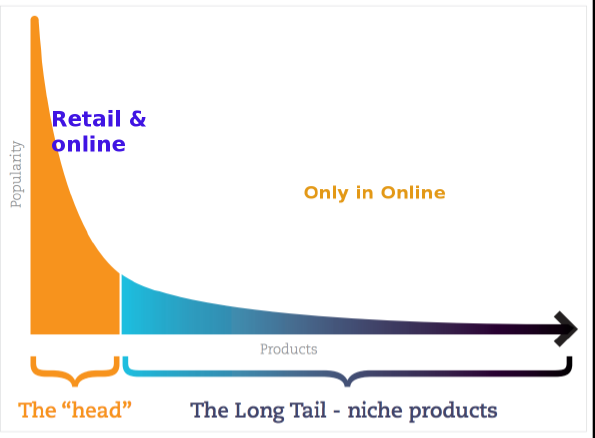
\includegraphics[width=2.5in]{longtailphenomenon}
		\caption{longtailphenomenon}
		\label{fig:longtailphenomenon}
	\end{figure}


	\begin{bulletedlist}
		\item Why Recommendation Systems?
		\begin{bulletedlist}
			\item Help user find item of their interest.
			\item Help item provider deliver their items to right user.
			\begin{bulletedlist}
				\item Identify products most relevant to the user
				\item Personalized content
				\item Eg. Top n offers
			\end{bulletedlist}
			\item Help website improve user engagement
		\end{bulletedlist}
		\item Recommender system creates a matching between users and items and exploits the similarity between users/items to make recommendations.
		\item What can be recommended?
		\begin{bulletedlist}
			\item Advertising messages, Movies, Books, Music tracks, News articles, Restaurants, Future friends (Social network sites), Courses in e-learning, Jobs, Research papers, Investment choices, TV programs, Citations, Cloths, Online mates (Dating services), Supermarket goods
		\end{bulletedlist}
		\item User and matching items
		\begin{bulletedlist}
			\item Amazon Users: members, Items: products, books etc. (35\% sales are from recommendation)
			\item Netflix Users: members, Items: movies, TV shows (2/3 rented movies are from recommendation)
			\item LinkedIn Users: members, Items: members
			\item Facebook Users: members, Items: job
			\item Google News (a38\% more click-through are due to recommendation)
		\end{bulletedlist}
	\end{bulletedlist}

	\section{Recommendation Historical Trends}
In 1988, Mr. Joe Simpson, an English mountain climber, wrote a book called \textit{Touching the Void}.  It got good reviews but was considered as modest success and it was soon forgotten.

However, a decade later, an interesting thing happened. Mr. Jon Krakauer wrote a book called \textit{Into Thin Air}, a thriller about a
mountain-climbing tragedy, which became a publishing sensation. Suddenly, \textit{Touching the Void} started to sell again.

Real world examples

	\begin{bulletedlist}
		\item GroupLens(https://grouplens.org/)
		\begin{bulletedlist}
			\item Helped in development of initial recommender systems by pioneering initial collaborative filtering models.
			\item Provided various data sets - MovieLens and BookLens.
		\end{bulletedlist}
		\item Amazon - Did lot of work on implementing commercial recommender systems
		\begin{bulletedlist}
			\item They also implemented lot of computational improvements.
		\end{bulletedlist}
		\item Netflix Prize
		\begin{bulletedlist}
			\item Pioneered Latent Factor/Matrix Factorization models
		\end{bulletedlist}
		\item Google - You Tube
		\begin{bulletedlist}
			\item Hybrid recommendation systems.
			\item Deep Learning Based Systems.
		\end{bulletedlist}
		\item Social Network Recommendations.
	\end{bulletedlist}

Perfect matching item may not exist (see \figurename~\ref{fig:imperfectmatchrecommendationsystem}).

	\begin{figure}[tbh]
		\centering
		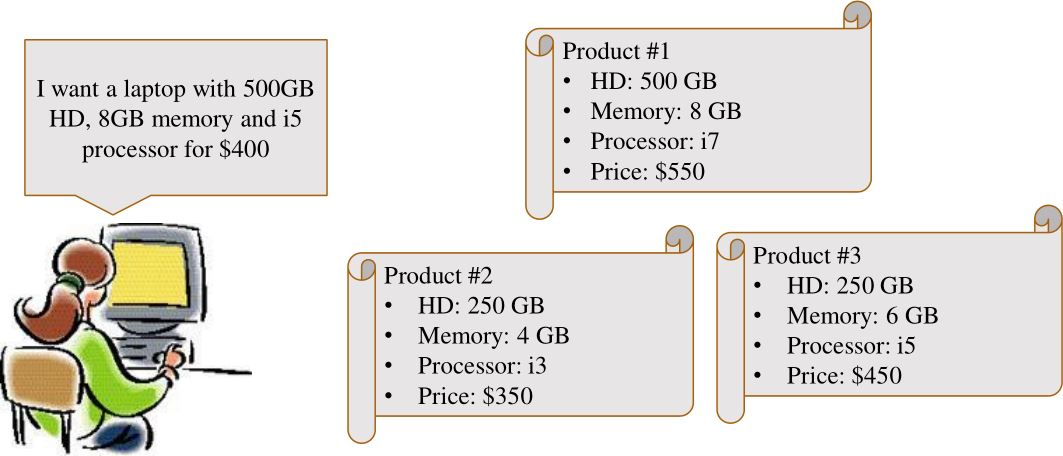
\includegraphics[height=2in]{imperfectmatchrecommendationsystem}
		\caption[Perfect matching recommendation may not exist]{Perfect matching recommendation may not exist.}
		\label{fig:imperfectmatchrecommendationsystem}
	\end{figure}

Types of recommendation systems
	\begin{bulletedlist}
		\item Popularity based recommendations
		\item Classification model based
		\item Content based recommendations
		\item Nearest neighbor collaborative filtering:
		\begin{bulletedlist}
			\item User based
			\item Item based
		\end{bulletedlist}
		\item Hybrid approaches
		\item Association rule mining
	\end{bulletedlist}

Popularity based Recommender System
	\begin{bulletedlist}
		\item Popularity based recommendation system works by recommending items viewed/pur\-chased by most people and rated high.
		\item Recommendations: Ranked list of items by their purchase count/viewed count.
		\item``Popular News''
		\begin{bulletedlist}
			\item Can use context
			\item Purchase history
			\item User and item features
			\item Scalable
		\end{bulletedlist}
		\item Not a personalized recommendation
	\end{bulletedlist}

	\section{Classification model}
	\begin{bulletedlist}
		\item Uses features of both products as well as users in order to predict whether a user will like a product or not.
		\item Limitation
		\begin{numberedlist}
			\item It is not easy to collect quality information about products and users.
			\item Even if we are able to collect good information, they may not be sufficient to make a good classifier.
			\item Scalability issue.
		\end{numberedlist}
	\end{bulletedlist}

	\begin{figure}[tbh]
		\centering
		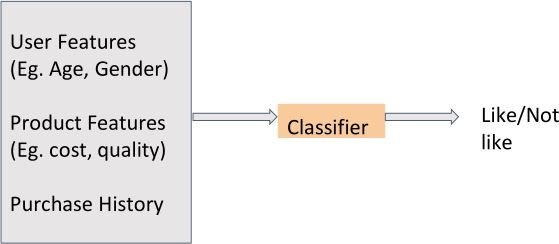
\includegraphics[height=2in]{recommendationsystemsclassificationmodel}
		\caption[Classification model]{Classification model.  The outcome can be 1 if the user likes it else 0 and it incorporates personalization.}
		\label{fig:recommendationsystemsclassificationmodel}
	\end{figure}

	\section{Content Based Recommendations}

	\begin{bulletedlist}
		\item Recommendations are based on information on the content of items rather than on other users' opinions.
		\item Main idea:
		\item If a user likes an item then he/she will also like a “similar” item
		\item Recommend items based on their similarity:
		\begin{bulletedlist}
			\item Recommend items to customer x similar to previous items rated highly by x.
		\end{bulletedlist}
		\item No need for data on other users.
		\begin{bulletedlist}
			\item No cold-start or sparsity problems.
		\end{bulletedlist}
		\item Able to recommend to users with unique tastes.
		\item Techniques that can be used: Cosine similarity.
	\end{bulletedlist}

	\section{Content Based Recommendation System}

	\begin{bulletedlist}
		\item Item Profiles:
		\begin{bulletedlist}
			\item set of features
			\item vector
		\end{bulletedlist}
		\begin{bulletedlist}
			\item Weighted average of rated item profiles
			\item Normalize rating using average rating of user.
		\end{bulletedlist}
		\item Advantages
		\begin{bulletedlist}
			\item Content-based recommender systems don't require a lot of user data.
			\item We just need item data and you're able to start giving recommendations to users.
			\item Recommendation engine does not depend on lots of user data, so it is possible to give recommendations to even your first customer as long as you have adequate data to build his user profile. Does not suffer from cold start.
			\item Less expensive to build and maintain.
		\end{bulletedlist}
		\item Challenges
		\begin{bulletedlist}
			\item Your item data needs to be well distributed.
			\item Availability of features which explain Items and user preferences.
			\item Recommendations will likely be direct substitutes, and not complements, of the item the user interacted with.  This is one of the key reasons why collaborative filtering provides better recommendations.
			\item Less dynamic.
		\end{bulletedlist}
	\end{bulletedlist}

	\begin{figure}
		\centering
		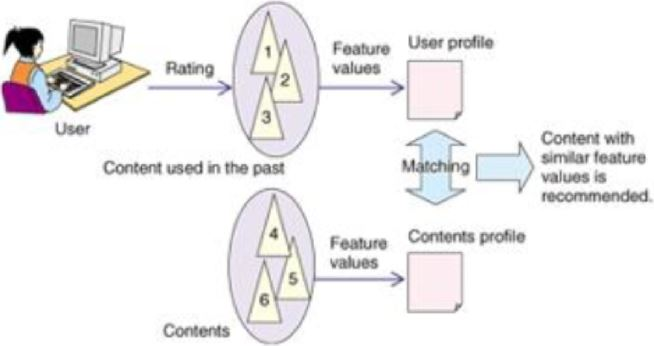
\includegraphics[width=2in]{contentbaserecommendationsystem}
		\caption[Content based recommendation system]{Content based recommendation system.}
		\label{fig:contentbaserecommendationsystem}
	\end{figure}

	\section{Cosine Similarity}
	\begin{bulletedlist}
		\item Cosine Similarity is the cosine of the angle between the 2 vectors A and B
		\item Closer the vectors, smaller will be the angle and hence larger their cosine value.
	\end{bulletedlist}

	\begin{equation}\label{eqn:cosinesimilarity}
		CosSim(x,y) = \frac{\sum_i x_i y_i}{\sqrt{\sum_i x_i^2}\sqrt{\sum_i y_i^2}} = \frac{\langle x,y\rangle}{\|x\|\|y\|}
	\end{equation}

	\chapter{Prompt Engineering}

\section{Azure OpenAI Access}
Microsoft instructions: \href{https://learn.microsoft.com/en-us/training/modules/get-started-openai/1-introduction}{Getting started with OpenAI}.

\section{Effective Prompts}
Effective system prompt:
\begin{numberedlist}
	\item Define the role.
	\item Define the objective/goal
	\item Any constraints/any specific rules
	\item Output format (bullet points, JSON, YAML)
\end{numberedlist} 

\section{Evaluation Metrics for Summarization}
\subsection{Introduction}
In order to evaluate model predictions (i.e., AI generated summaries), we compare the model predictions with the ground truth on a sample of human-annotated gold examples. However, given the subjective nature of model predictions, we need new metrics to evaluate summarization outputs: ROUGE and BERT Score.

\subsection{Recall-Oriented Understudy for Gisting Evaluation (ROUGE)}
What is ROUGE?
\begin{bulletedlist}
	\item ROUGE is a set of metrics that measure the similarity between a candidate summary and a set of reference summaries by comparing the grams (tokens, characters or words) present in them.
	\item The ROUGE score ranges from 0 to 1, with a score close to 1 indicating strong similarity between the candidate and reference summaries.
	\item Higher ROUGE scores indicate better performance in preserving key information from the original text while generating a concise summary
\end{bulletedlist}

Because it depends on the presence of exact matches, ROUGE is better fit for extractive summarization than abstractive.

\subsubsection{What is N-grams in ROUGE?}
\begin{bulletedlist}
	\item N-grams are a fundamental concept in Natural Language Processing (NLP). They are used to analyze and understand the structure of text by identifying sequences of n items (words, characters, or phonemes) from a given text.
	\item The term "n" in n-grams represents the size of the sequence (number of words), which can be any positive integer.
	\item ROUGE measure the overlap of n-grams between the system and reference summaries. N-grams refer to sequences of n items (words, characters, or phonemes) from a given text.
	\item The ROUGE metric is designed to capture the recall-oriented aspects of summarization, focusing on the ability of the generated summary to capture the essential information from the source text.
\end{bulletedlist}

\subsubsection{Types of ROUGE}
There are several variants of the ROUGE metric:
\begin{bulletedlist}
	\item ROUGE-N: Measures the overlap of n-grams (sequences of n words) between the system and reference summaries. For example, ROUGE-1 refers to the overlap of unigrams (single words), while ROUGE-2 refers to the overlap of bigrams (pairs of words).
	\item ROUGE-L: ROUGE-L, also known as ROUGE-LCS, focuses on the Longest Common Subsequence (LCS) between a system-generated summary and a reference summary. It aims to balance precision and recall by calculating a weighted harmonic mean, known as the F-measure.
	\begin{bulletedlist}
		\item LCS Importance: ROUGE-L considers the longest sequence of words shared between the system and reference summaries, allowing for non-consecutive matches that reflect sentence-level word order.
		\item Precision and Recall: It combines precision (correctness) and recall (completeness) to provide a comprehensive evaluation of summary quality.
	\end{bulletedlist}
	\item ROUGE-W: Both ROUGE-W and ROUGE-L are based on the longest common subsequence, while The key idea behind ROUGE-W is to assign higher weights to consecutive matches in the LCS, favoring summaries that maintain the order of words from the reference text.
	\item ROUGE-S is a metric used to evaluate the quality of automatically generated summaries by focusing on skip-bigrams. Skip-bigrams considers pairs of words that maintain their sentence order but may have other words in between, capturing the essence of sentence-level structure.
\end{bulletedlist}

\subsubsection{Example}
A common variant of ROUGE that is used to generate a comparison metric is ROUGE-L , where we first compute the recall and precision of the longest common subsequence and then compute the harmonic mean of these values (punctuation and case of the word are disregarded). 

 	\begin{figure}
		\centering
		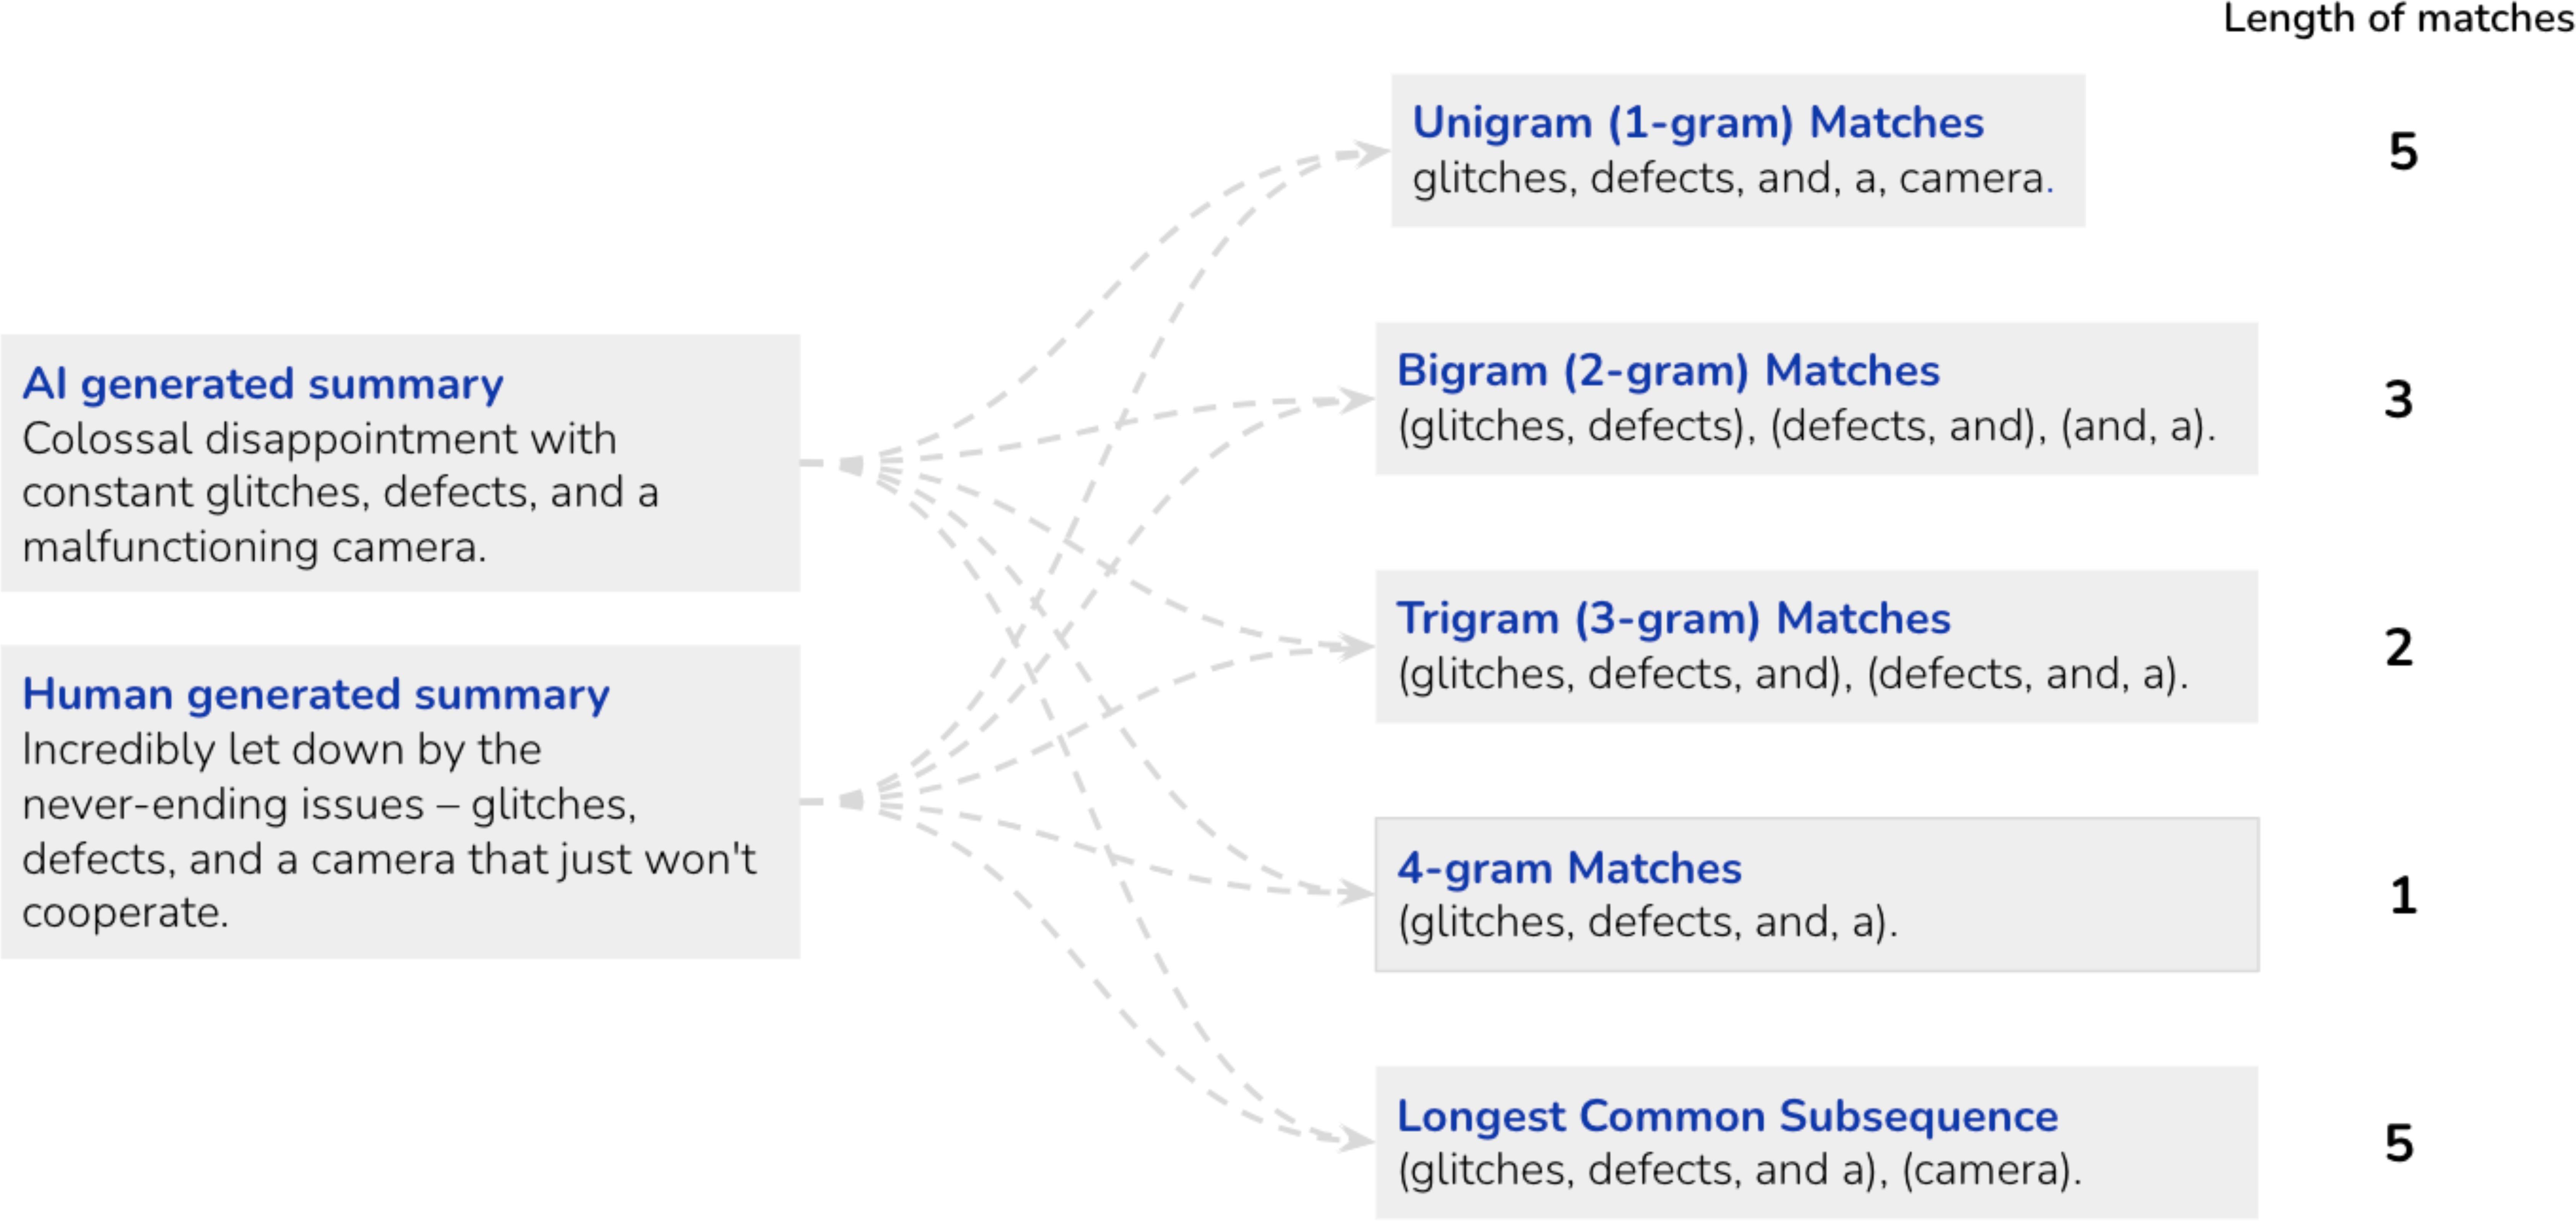
\includegraphics[width=5.0in]{summarizationmetricrouge}
		\caption[ROUGE N-grams]{ROUGE N-grams.}
		\label{fig:summarizationmetricrouge}
	\end{figure}


ai\_generated\_summary = "Colossal disappointment with constant glitches, defects, and a malfunctioning camera."
human\_generated\_summary = "Incredibly let down by the never-ending issues – glitches, defects, and a camera that just won't cooperate."

As seen in the figure above, the length of the largest common subsequence (LCS) between the two summaries is 5. The number of unigrams in the AI-generated summary is 10 and the number of unigrams in the human generated summary is 17.

We define the recall of the LCS as 5/17 and the precision of the LCS as 5/10 (notice the parallel with the precision and recall measures used to evaluate classification tasks).

From these measures, we can compute ROUGE-L as the F1 score associated with the precision and recall like so:

%r_lcs = 5/17
%p_lcs = 5/10
%
%(2 * r_lcs * p_lcs)/(r_lcs + p_lcs) # Rouge-L
 

ROUGE is effective in scenarios involving abstractive summarization tasks, automatic summarization evaluation, assessments of large language models (LLMs), and comparative analyses of different summarization approaches. However, ROUGE lacks semantic understanding and doesn't evaluate whether the system truly understood the meanings and concepts in the original text. This can be addressed by the next metrics which is BERT Score.

2. BERT Score
What is BERT Score?
The BERT Score is a novel automatic evaluation metric for text generation tasks, such as summarization, machine translation, and image captioning. It leverages the pre-trained contextual embeddings from BERT (Bidirectional Encoder Representations from Transformers) to measure the semantic similarity between the candidate (system-generated) and reference (ground truth) sentences.
Key Idea:

Embeddings: BERT Score uses the contextual embeddings from BERT to capture the semantic meaning of words in both the candidate and reference sentences.
Semantic Similarity: It computes the similarity between each word in the candidate sentence and each word in the reference sentence based on their contextual embeddings.
Precision, Recall, and F1 Score: BERT Score calculates precision, recall, and the F1 score based on the maximum similarity for each word, providing a comprehensive evaluation of the generated text
What are Embeddings in BERT Score?

Embeddings are a way for computers to understand the meaning of words based on the words around them. It's like when you read a sentence, you can figure out what a word means by looking at the other words in the sentence.

\noindent{}Example:
\begin{plainlist}
\item \textcode{\Small{} ai\_generated\_summary = ``Major issues, malfunctioning camera.''}
\item \textcode{\Small{} human\_generated\_summary = ``Severely disappointed, constant problems.''}
\end{plainlist}
Look at the two summaries presented above. Though the choice of words is not exactly the same, both are close in intent.
In order to capture intent, we use specific models that encode the semantic meaning of words used in the models in a mathematical space where we can measure the distance between the words used.
Since distances can be computed, if two words are close to each other in this mathematical space (i.e., less distance), we can infer that these two words are close in meaning.
What are Embedding Models?

Models that encode the word mappings, that is, models that associate words with a list of numbers (called vectors) that define positions of the words in a mathematical space are referred to as embedding models. 
Embedding models are precursors to language models and are a crucial component of how we represent the semantic meaning of words used in text. For example, here glitches, problem and issues are the related words and will have similar representation in the model. 


So we can see that BERT Score provides a more nuanced evaluation by considering semantic similarity and context. However, BERT Score can be computationally intensive due to its reliance on pre-trained language models

\subsection{Conclusion}
In summary, both ROUGE and BERT Score have their strengths and weaknesses in evaluating text summarization systems. ROUGE offers a baseline for content selection, while BERT Score provides a more comprehensive assessment of semantic similarity and alignment with human judgments. The choice between the two metrics depends on the specific requirements of the summarization task and the desired level of granularity in the evaluation process. 

	\appendix{}
	\input{"Interview Questions"}
	\input{"Installation Notes"}

	\backmatter{}
	\pagestyle{leplainheader}



%	% Standard glossary entries.
%	\newglossaryentry{utc}{name=UTC, description={Coordinated Universal Time}}
%	%\gls{utc}
%	\printglossary[type=main, title=General Glossary]{}
%	\renewcommand*{\chaptertitle}{General Glossary}

	% Statistics glossary.
	\printglossary[type=stats, title=Statistics Glossary]{}
	\renewcommand*{\chaptertitle}{Statistics Glossary}

	% Modeling glossary.
	\printglossary[type=model, title=Modeling Glossary]{}
	\renewcommand*{\chaptertitle}{Modeling Glossary}

	% Acronyms.
	\printglossary[type=\acronymtype]
	\renewcommand*{\chaptertitle}{Acronyms}

	% PRINT A LIST OF NOTATIONS / NOMENCLATURE.
	% Argument is a text/tex file containing lines in the form of:
	% \addnotation{Variable}{Meaning of variable.}
	\input{"List of Notations.tex"}

	% Use all glossary entries without specifically referencing them.
	% Gather all unused glossary terms.  Putting it before "\printgossaries" seems to cause a blank page to be injected.
	\glsaddallunused{}

	\bibliography{le, machinelearning}

	\end{document}
